\documentclass[9pt]{beamer}
% Created By Gouthaman KG
%~~~~~~~~~~~~~~~~~~~~~~~~~~~~~~~~~~~~~~~~~~~~~~~~~~~~~~~~~~~~~~~~~~~~~~~~~~~~~~
% Use roboto Font (recommended)
\usepackage[sfdefault]{roboto}
\usepackage[utf8]{inputenc}
\usepackage[T1]{fontenc}
\usepackage[absolute,overlay]{textpos}
%~~~~~~~~~~~~~~~~~~~~~~~~~~~~~~~~~~~~~~~~~~~~~~~~~~~~~~~~~~~~~~~~~~~~~~~~~~~~~~

%~~~~~~~~~~~~~~~~~~~~~~~~~~~~~~~~~~~~~~~~~~~~~~~~~~~~~~~~~~~~~~~~~~~~~~~~~~~~~~
% Define where theme files are located. ('/styles')
\usepackage{styles/fluxmacros}
\usefolder{styles}
% Use Flux theme v0.1 beta
% Available style: asphalt, blue, red, green, gray 
\usetheme[style=asphalt]{flux}
%~~~~~~~~~~~~~~~~~~~~~~~~~~~~~~~~~~~~~~~~~~~~~~~~~~~~~~~~~~~~~~~~~~~~~~~~~~~~~~

%~~~~~~~~~~~~~~~~~~~~~~~~~~~~~~~~~~~~~~~~~~~~~~~~~~~~~~~~~~~~~~~~~~~~~~~~~~~~~~
% Extra packages for the demo:
\usepackage{booktabs}
\usepackage{colortbl}
\usepackage{ragged2e}
\usepackage{schemabloc}
\usepackage{hyperref}
\graphicspath{{./assets/}}

\usebackgroundtemplate{

\includegraphics[width=\paperwidth, height=\paperheight]{assets/background.pdf}}%change this to your preferred background for the presentation.
%~~~~~~~~~~~~~~~~~~~~~~~~~~~~~~~~~~~~~~~~~~~~~~~~~~~~~~~~~~~~~~~~~~~~~~~~~~~~~~

%~~~~~~~~~~~~~~~~~~~~~~~~~~~~~~~~~~~~~~~~~~~~~~~~~~~~~~~~~~~~~~~~~~~~~~~~~~~~~~

% Other packages:
\usepackage{mhchem}
\usepackage{transparent}
\usepackage{media9}
\usepackage{graphicx}
\usepackage{gensymb}
%~~~~~~~~~~~~~~~~~~~~~~~~~~~~~~~~~~~~~~~~~~~~~~~~~~~~~~~~~~~~~~~~~~~~~~~~~~~~~~
% Informationsm
\title{\textsc{Follow-up Meeting}}
\subtitle{\textbf{Jorge Romero}}

\author{\textbf{Jyväskylän Yliopisto}}
\institute{5. huhtikuuta 2021}
\titlegraphic{assets/logo_white.pdf} %change this to your preferred logo or image(the image is located on the top right corner).
%~~~~~~~~~~~~~~~~~~~~~~~~~~~~~~~~~~~~~~~~~~~~~~~~~~~~~~~~~~~~~~~~~~~~~~~~~~~~~~

\begin{document}
% Generate title page
\titlepage

% \begin{frame}{TABLE OF CONTENTS}
% \frametitle{TABLE OF CONTENTS}
%  \tableofcontents
% \end{frame}
\begin{frame}{\textsc{Dual Doctoral Programme}}
    \begin{textblock*}{5cm}(0.5cm,2cm)
        \centering
        
\includegraphics[width=\textwidth]{liverpool-logo.pdf}
        \begin{itemize}
            \item<2-> Year 1: Oct 2019 - Sep 2020
            \item<4-> Year 4: Oct 2022 - Sep 2023*
        \end{itemize}
    \end{textblock*}
    \begin{textblock*}{5cm}(7cm,1.25cm)
        \centering
        
\includegraphics[width=\textwidth]{jyu-vaaka-kaksikielinen.eps}
        \begin{itemize}
            \item<3-> Year 2\&3: Sep 2020 - Sep 2022             
        \end{itemize}
    \end{textblock*}
    
    \begin{textblock*}{5cm}(0.5cm,5.5cm)
        \onslide<5->{\Large \textbf{Project}}

        \onslide<5->{Investigation of exotic nuclei close to the proton drip line using the state-of-the-art MARA-LEB facility.}

    \end{textblock*}

    \begin{textblock*}{5cm}(5cm,5cm)
        
            \includegraphics<5->[scale=0.4]{ROI.pdf}

    \end{textblock*}
\end{frame}

\begin{frame}{\textsc{Physics Courses}}
    \begin{textblock*}{12cm}(0.5cm,1.1cm)
    {\Large \textbullet \textbf{Discipline-Specific Skills}}
        
    \vspace{1em}
    Completed

    {\centering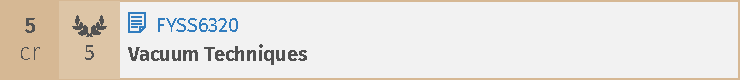
\includegraphics[scale=0.75]{vacuum.pdf}}

    \onslide<2->{Starting next year:}

     {\centering   \includegraphics<2->[scale=0.75]{accelerator.pdf}
        \includegraphics<2->[scale=0.75]{laser.pdf}}

    \onslide<3->{Starting next year:}

    {  \includegraphics<3->[scale=0.75]{models.pdf}}

    \begin{center}
        \onslide<4->{\textbf{Physics Credit Total: 24/40 cr}}
    \end{center}
    \end{textblock*}    
\end{frame}

\begin{frame}{\textsc{Transferable Skills Courses}}
    \begin{textblock*}{12cm}(0.5cm,1.1cm)
    {\Large \textbullet \textbf{Research Competence Courses}}

    Compulsory course (completed):
    {\centering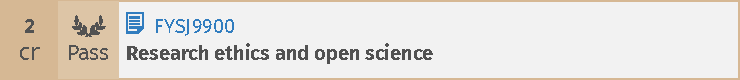
\includegraphics[scale=0.75]{ethics.pdf}}

    \onslide<2->{{\Large \textbullet \textbf{Communication Skills Courses}}

     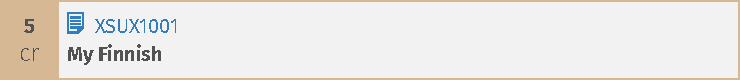
\includegraphics[scale=0.75]{finnish.pdf}}

    \onslide<3->{{\Large \textbullet \textbf{Other Competence}}

     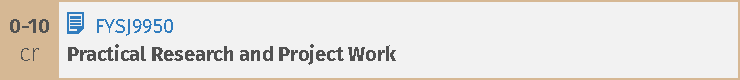
\includegraphics[scale=0.75]{practical.pdf}
     
     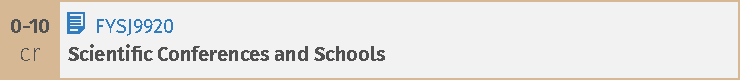
\includegraphics[scale=0.75]{conference.pdf}}

     \begin{center}
        \onslide<4->{\textbf{Non-Physics Credit Total: Up to 27/40 cr}}
    \end{center}

    \end{textblock*}    
\end{frame}

\begin{frame}{\textsc{Experiment M17}}
    \begin{textblock*}{12cm}(0.5cm,1.5cm)
        Experiment using MARA in November 2020. 

        Reactions of interest $$\ce{^{40}Ca}(\ce{^{58,60}Ni}, p3n)\ce{^{94,96}Ag}$$
        \begin{flushright}
            \onslide<2->{$\Rightarrow$ Closer Analysis in progress to obtain information on Ag (Interest for MARA-LEB).}
        \end{flushright}

       \onslide<3->{ $\Rightarrow$ Analysis of A=96 recoils distribution at MARA focal plane performed to study transmission into MARA-LEB gas cell as a function of window size.} \onslide<4->{$\Rightarrow$ \textbf{Shown within poster for Physics Days 2021}.}
    \end{textblock*}    
    \begin{textblock*}{12cm}(0.5cm,5.1cm)
        \includegraphics<3->[scale=0.23]{window.pdf} \hfill \includegraphics<4->[scale=0.1]{qr-code.pdf}        
    \end{textblock*} 
\end{frame}

\begin{frame}{\textsc{Simulations}}
    \begin{textblock*}{12cm}(0.5cm,2.5cm)
        \onslide<1>{Performing simulations using Simion to study transmission rates through the MARA-LEB RFQs for different parameters. Working together with Wouter Gins.} 
    \end{textblock*}    
        
    \begin{textblock*}{12cm}(0.5cm,1.5cm)
            \includegraphics<1>[angle=20,scale=0.3]{RFQ.pdf}
    \end{textblock*}    

    \centering
    \includegraphics<2>[scale=0.6]{transmission_matrix.jpg}
    

\end{frame}


\end{document}